%\documentclass[12pt,a4paper]{book}
%\usepackage{commands}
%
%\begin{document
%
%	
%\end{document}
\documentclass{labdiary}
\usepackage{commands}
\usepackage{natbib} 
%\setcitestyle{authoryear, open={([},close={)]}}
%\setcitestyle{numbers,square}
\bibliographystyle{dinat}



%\includeonly{Chapters/theoriticalInvestiagtion}
\title{Hierarchical Self-Assembly}
\author{Ali Fele Paranj}
\date{\today}

\begin{document}
	
%	\maketitle
	
	
	\begin{tikzpicture}[remember picture,overlay]
		% If a chapter image has been specified
		%         \expandafter\ifstrequal\expandafter{Images/vendingMachine.png}{}{}{
			% Output the chapter image
			\node[
			anchor=north west, % Anchor point on the image
			inner sep=0pt, % Inner padding
			] at (current page.north west) {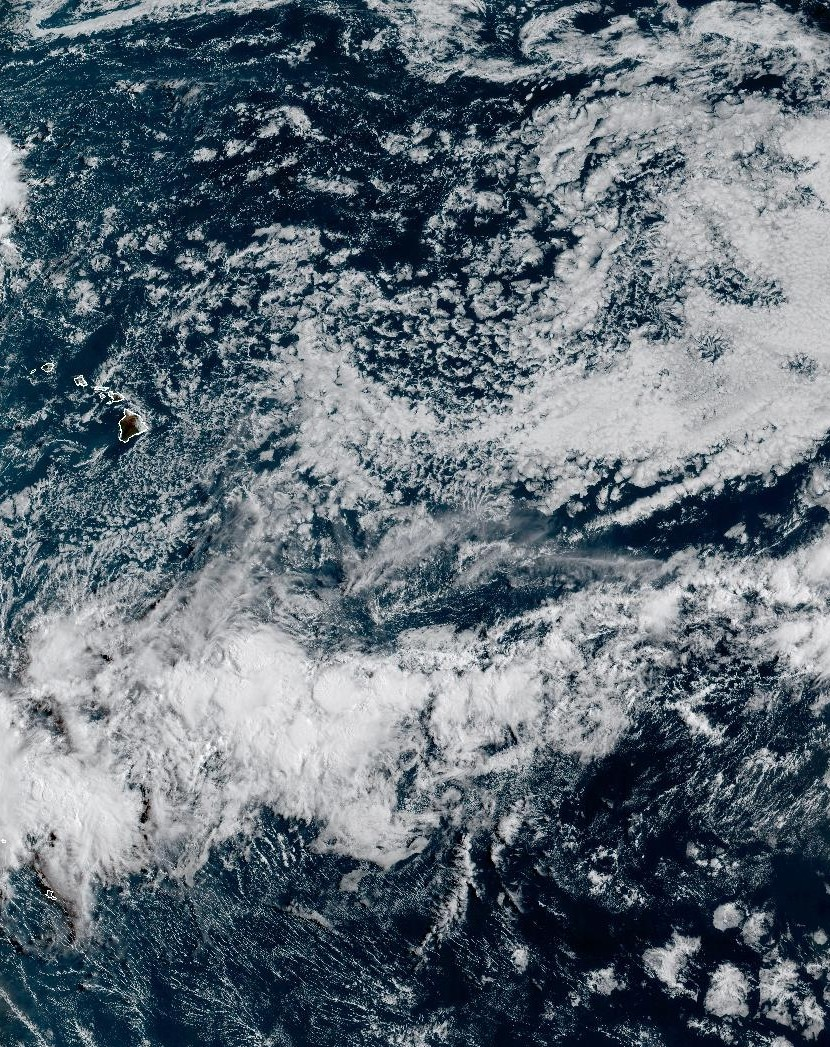
\includegraphics[angle=0,height=\paperheight]{images/scalefree.jpg}};
			%	         }
	\end{tikzpicture} 
	
	
	\vspace{-0cm}
	\heading{Hierarchical Self-Assembly}
	
	\newpage
	
	
	
	\tableofcontents
	
%	\include{Chapters/StatisticalPhysicsForBiology.tex}

	
	
	\part{Discrete Mathematics}
	\chapter{Combinatorics}


\section{Basic Review}

\begin{summary}
	One possible interpretation for the formula of $ n $-choose-$ k $ is the following. Let $ A = \set{a,b,c,d,e} $, and assume we want to choose $ 2 $ elements from the set. Fix some ordering for the elements in the set and assume each selection is represented by a 5-tuple, where each index specifies if that elements in the set is chosen. For instance $ (1,1,0,0,0) $ corresponds to the choice $ \set{a,b} $. So the total number of such choices will be total number of ways that we can arrange two 1's and three 0's, which is
	\[ \frac{5!}{2! 3!}. \]
	So in general we can write
	\[ \frac{n!}{(n-k)! k!}. \]
\end{summary}




\section{Solved Problems}
\begin{problem}
	What is the number of choosing $ k $ objects out of $ n $, where order does not matter, but repetitions are allows.
\end{problem}
\begin{solution}
	This problem is very similar to the one in the thermal physics bo by Schroeder when studying the number of possible ways to distribute $ Q $ units of energy in $ N $ Einstein solids. 
	
	Let's consider a concrete example where we want to choose 3 objects from $ \set{a,b,c,d,e} $ with replacement and order is not important. Then assume each object in the set is a container, and we have 3 balls to put in containers (exactly the same as distribution energy units between Einstein solids). So the outcome $ aaa $ corresponds to putting all three balls in $ a $, and etc. One can represent each outcome with a dot-line diagram. For instance $\bullet\ \bullet\ \bullet\ |\ |\ |\ $ corresponds $ aaa $ outcome. Note that we have $ n-1 $ lines and $ k $ balls. So total number of ways to arrange these objects is
	\[ \frac{(n+k-1)!}{k!(n-1)!} = \binom{n+k-1}{k}. \]
\end{solution} 
\begin{remark}
	Interestingly, the Einstein solid problem, and number of ways that one can choose $ k $ scoops of ice-cream in a shop with $ n $ scoops of ice-cream is the same.
\end{remark}
	\chapter{CAT0CubeComplexes}

	\chapter{AlgebraicStructures}

	
	\part{Probability}
	\chapter{Probability}

	\chapter{StochasticProcesses}

	
	
	\part{Physics}
	\chapter{StatisticalPhysics}

	
	\part{Computing}
	\chapter{TheoryOfComputing}

	\chapter{StochasticSimulations}

	
	
	\part{Meetings}
	\chapter{Meetings with Miranda}
	

	
	
	

	\bibliography{References/references} % The filename of the .bib file (without the extension)

	

	
	
\end{document}
